
\documentclass[10 pt,usenames,dvipsnames, oneside]{article}
\usepackage{../../modelo-fracoes}
\graphicspath{{../../../Figuras/licao04/}}


\begin{document}

\begin{center}
  \begin{minipage}[l]{3cm}

\includegraphics[width=2cm]{../../../Figuras/logo}       
\end{minipage}\hfill
\begin{minipage}[r]{.8\textwidth}
 {\Large \scshape Atividade: Retângulos coloridos - quantos cabem?}  
\end{minipage}
\end{center}
\vspace{.2cm}

\ifdefined\prof
%Caixa do Para o Professor
\begin{goals}
%Objetivos específicos
\begin{enumerate}
\item       Reconhecer que as frações       $\frac{1}{2}$,
$\frac{2}{4}$,       $\frac{3}{6}$,       $\frac{4}{8}$,       $\frac{5}{10}$
e       $\frac{8}{16}$       são iguais a partir da observação das
representações destas frações em modelos de área retangulares.
\end{enumerate}

\tcblower

%Orientações e sugestões
\begin{itemize}
\item       Recomenda-se que esta atividade seja desenvolvida em grupos de
$2$       ou       $3$       alunos para que eles possam discutir as
soluções apresentadas, dentro do grupo, durante a condução da atividade.
\item       É importante, ao final da atividade, observar para os alunos que
uma mesma parte do retângulo (a região colorida de cinza) está sendo descrita
por frações com numeradores e denominadores diferentes (isto é, por frações
equivalentes) mas que, não obstante, por expressarem uma mesma quantidade, são
frações iguais.
\end{itemize}

Esta atividade possui     folhas para reprodução disponíveis no final do
livro.
\end{goals}

\bigskip
\begin{center}
{\large \scshape Atividade}
\end{center}
\fi

{\bf PARTE 1}

Você recebeu um encarte com 10 retângulos coloridos de mesmo tamanho, cada um deles dividido em um determinado número de partes iguais. Seguindo o modelo feito para o primeiro retângulo, preencha a tabela a seguir.


\begin{center}
\begin{longtable}{|c|m{.25\textwidth}|m{.25\textwidth}|}
\hline
\centering Retângulo  &   Número de partes em que se encontra dividido  &   Cada parte é que fração do retângulo?  \\
\hline
\endhead
\parbox[c][2cm][c]{.4\textwidth}{
\centering
\begin{tikzpicture}
\draw[fill=light] (0,0) rectangle (60,12);
\draw (30,0) -- (30,12);
\end{tikzpicture}}   &   \centering $2$ &  \centering $\dfrac{1}{2}$  \tabularnewline
\hline
\parbox[c][2cm][c]{.4\textwidth}{
\centering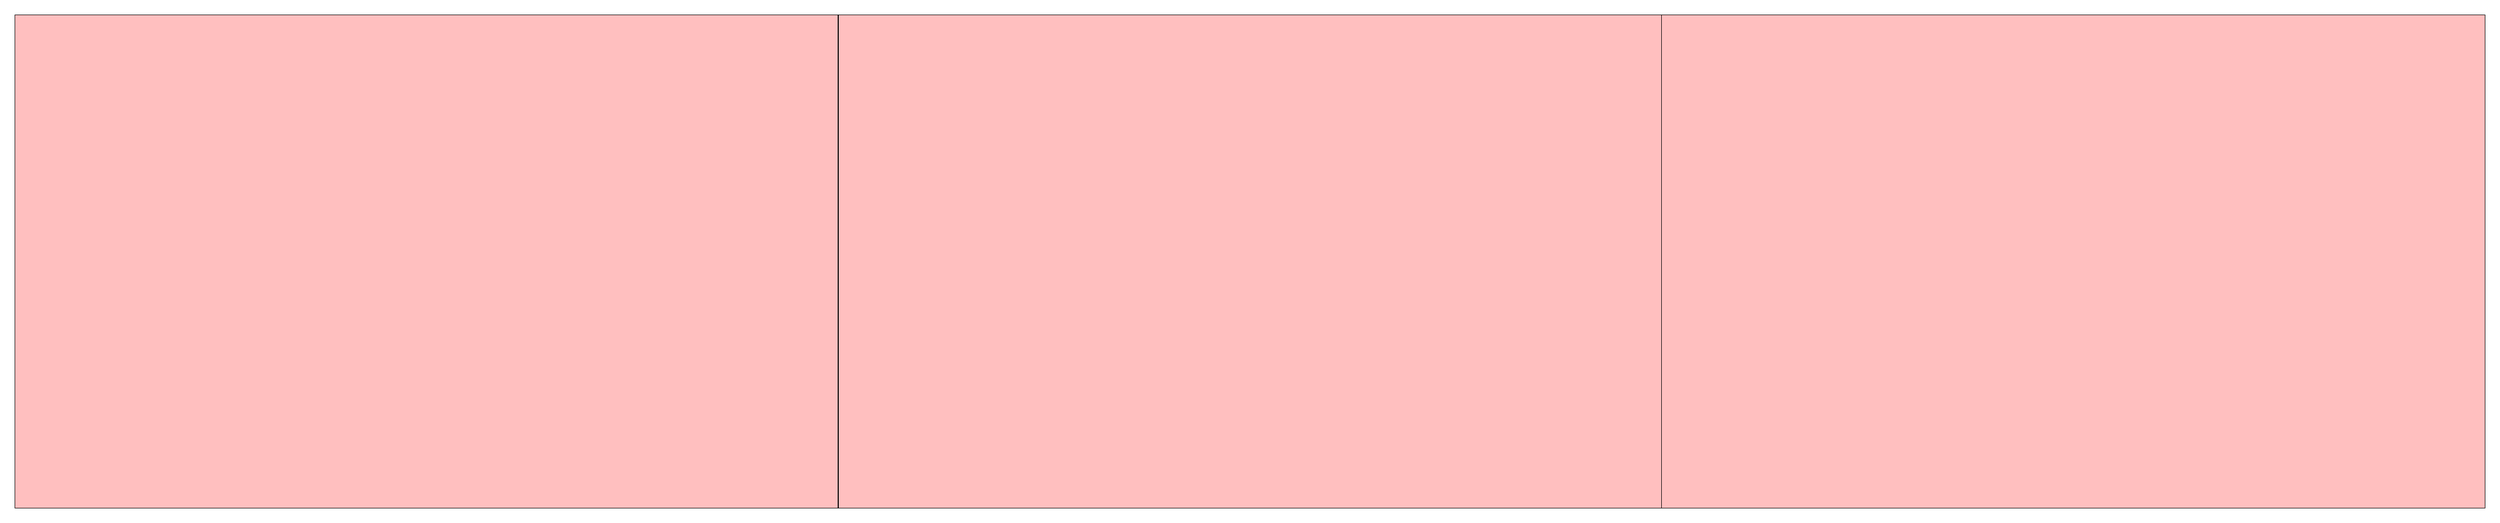
\begin{tikzpicture}
\draw[fill=pink] (0,0) rectangle (60,12);
\foreach \x in {1,2} \draw (\x*60/3,0) -- (\x*60/3,12);
\end{tikzpicture}}        &  \parbox[t][1.3 cm][c]{.2cm}{ }    &     \\
\hline
\parbox[c][2cm][c]{.4\textwidth}{
\centering\begin{tikzpicture}
\draw[fill=special] (0,0) rectangle (60,12);
\foreach \x in {1,2,3} \draw (\x*60/4,0) -- (\x*60/4,12);
\end{tikzpicture}}        &  \parbox[t][1.3 cm][c]{.2cm}{ }    &     \\
\hline
\parbox[c][2cm][c]{.4\textwidth}{
\centering\begin{tikzpicture}
\draw[fill=attention] (0,0) rectangle (60,12);
\foreach \x in {1,...,4} \draw (\x*60/5,0) -- (\x*60/5,12);
\end{tikzpicture}}        &  \parbox[t][1.3 cm][c]{.2cm}{ }    &     \\
\hline
\parbox[c][2cm][c]{.4\textwidth}{
\centering\begin{tikzpicture}
\draw[fill=common] (0,0) rectangle (60,12);
\foreach \x in {1,...,5} \draw (\x*60/6,0) -- (\x*60/6,12);
\end{tikzpicture}}        &  \parbox[t][1.3 cm][c]{.2cm}{ }    &     \\
\hline
\parbox[c][2cm][c]{.4\textwidth}{
\centering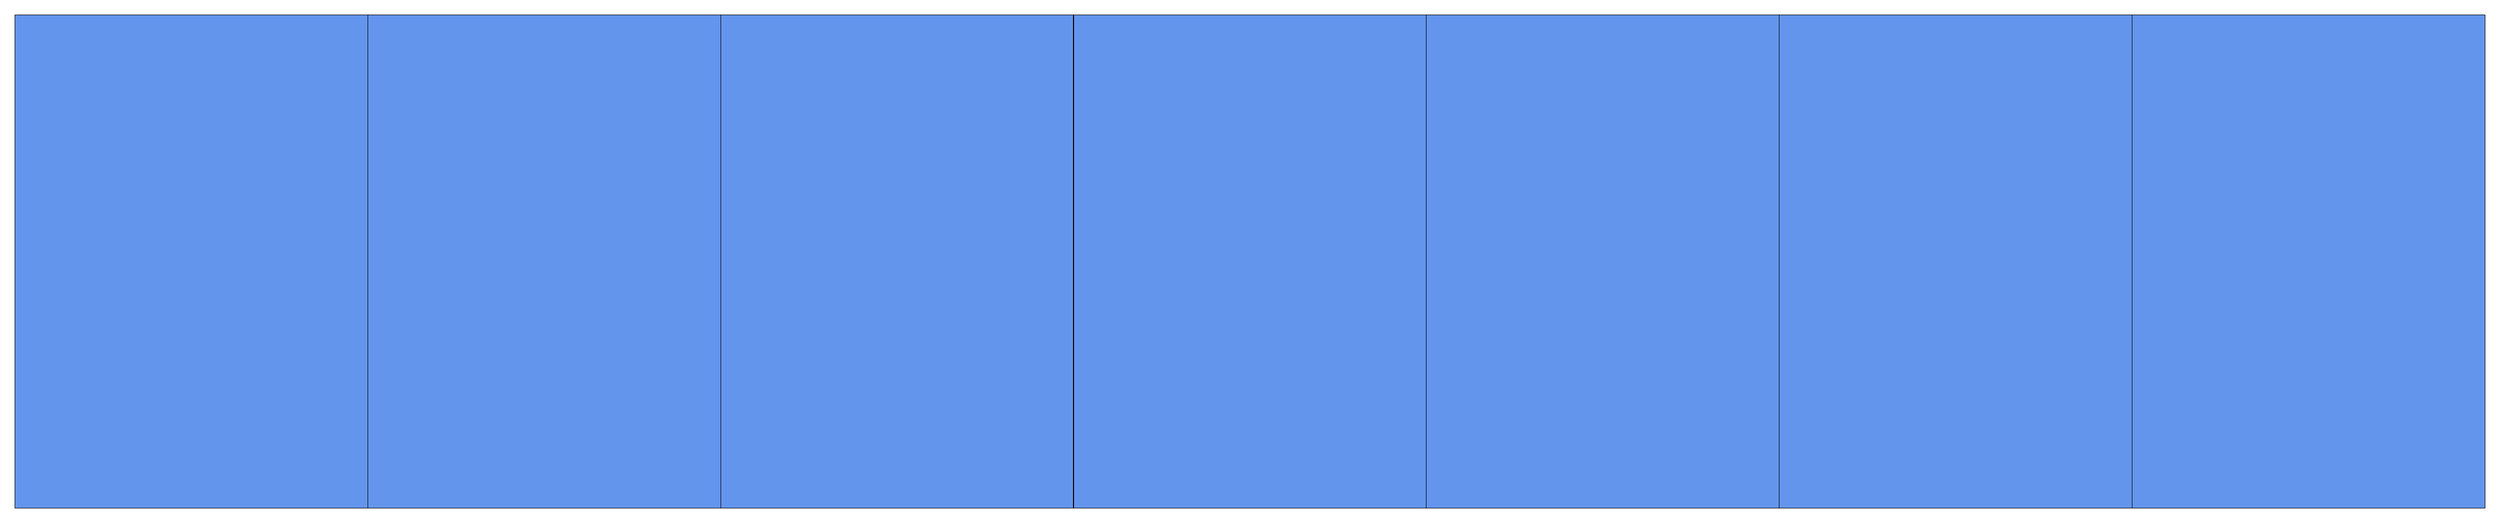
\begin{tikzpicture}
\draw[fill=CornflowerBlue] (0,0) rectangle (60,12);
\foreach \x in {1,...,6} \draw (\x*60/7,0) -- (\x*60/7,12);
\end{tikzpicture}}        &  \parbox[t][1.3 cm][c]{.2cm}{ }    &     \\
\hline
\parbox[c][2cm][c]{.4\textwidth}{
\centering\begin{tikzpicture}
\draw[fill=dark] (0,0) rectangle (60,12);
\foreach \x in {1,...,7} \draw (\x*60/8,0) -- (\x*60/8,12);
\end{tikzpicture}}        &  \parbox[t][1.3 cm][c]{.2cm}{ }    &     \\
\hline
\parbox[c][2cm][c]{.4\textwidth}{
\centering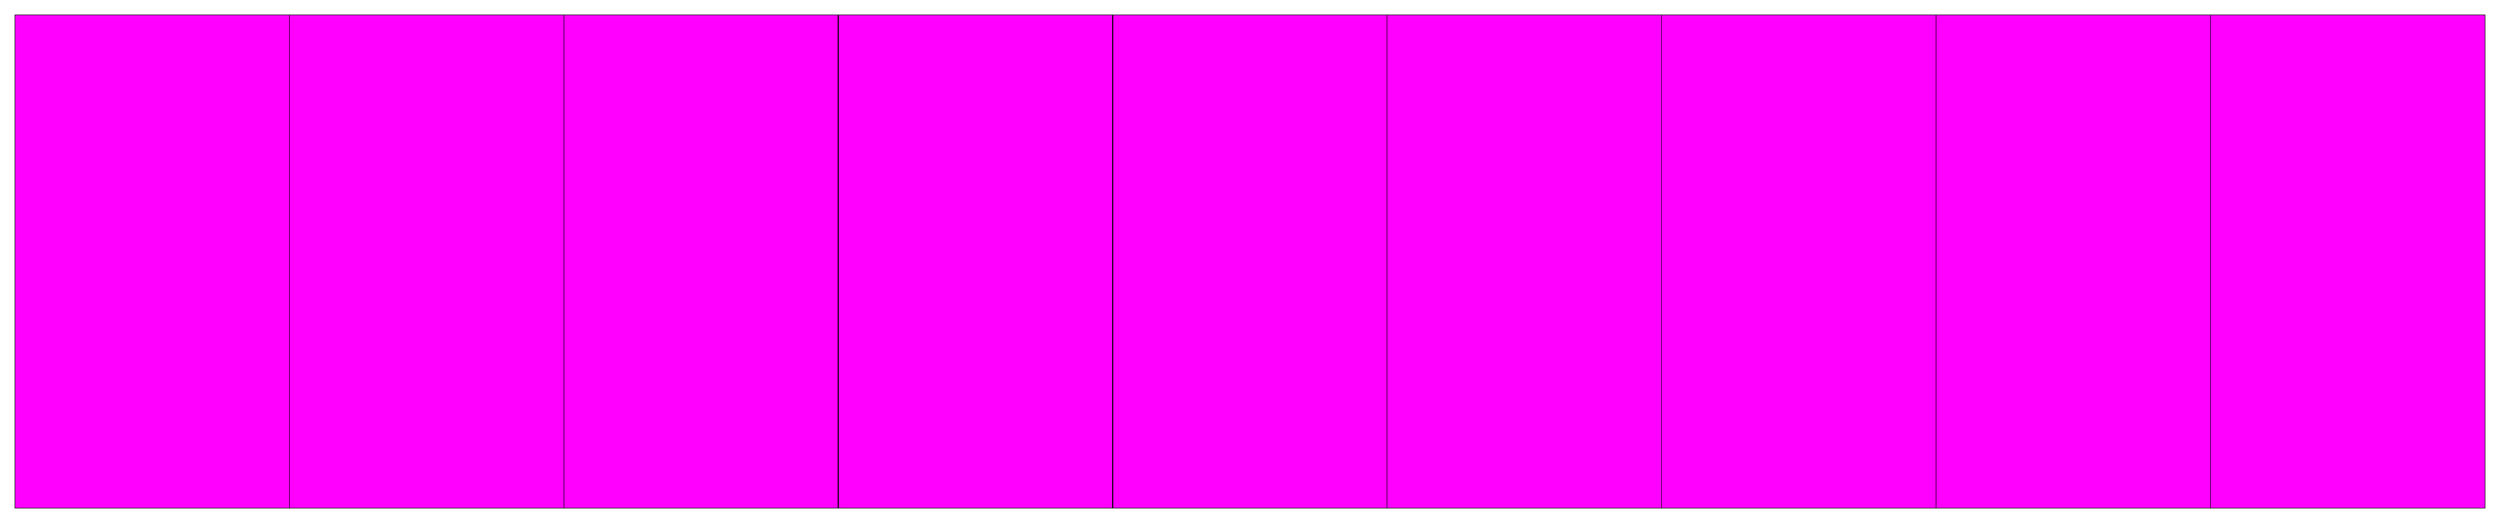
\begin{tikzpicture}
\draw[fill=Fuchsia] (0,0) rectangle (60,12);
\foreach \x in {1,...,8} \draw (\x*60/9,0) -- (\x*60/9,12);
\end{tikzpicture}}        &  \parbox[t][1.3 cm][c]{.2cm}{ }    &     \\
\hline
\parbox[c][2cm][c]{.4\textwidth}{\centering
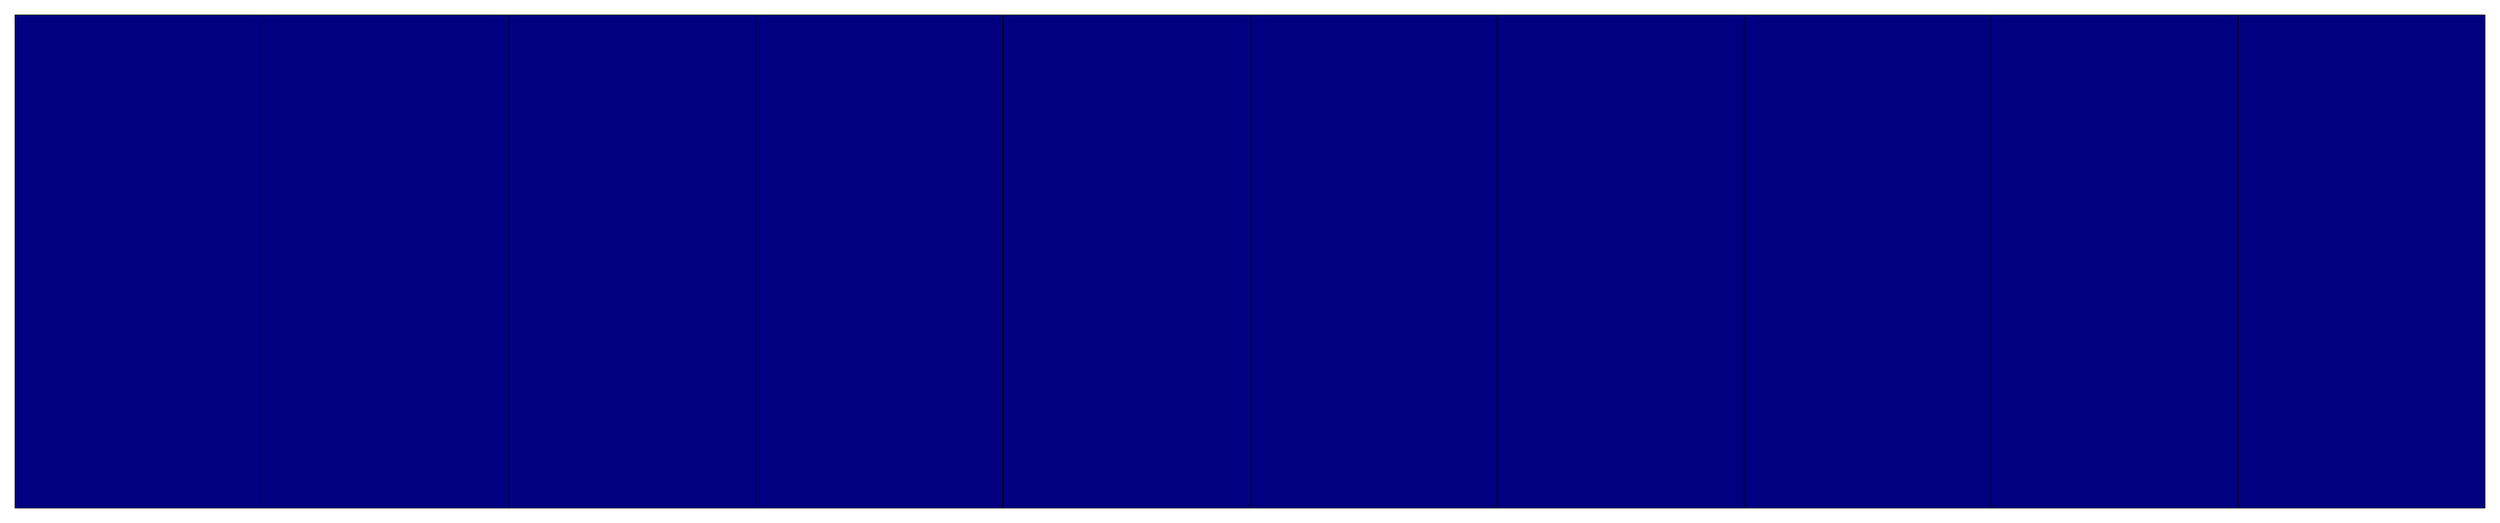
\begin{tikzpicture}
\draw[fill=NavyBlue] (0,0) rectangle (60,12);
\foreach \x in {1,...,9} \draw (\x*60/10,0) -- (\x*60/10,12);
\end{tikzpicture}}        &  \parbox[t][1.3 cm][c]{.2cm}{ }    &     \\
\hline
\parbox[c][2cm][c]{.4\textwidth}{\centering
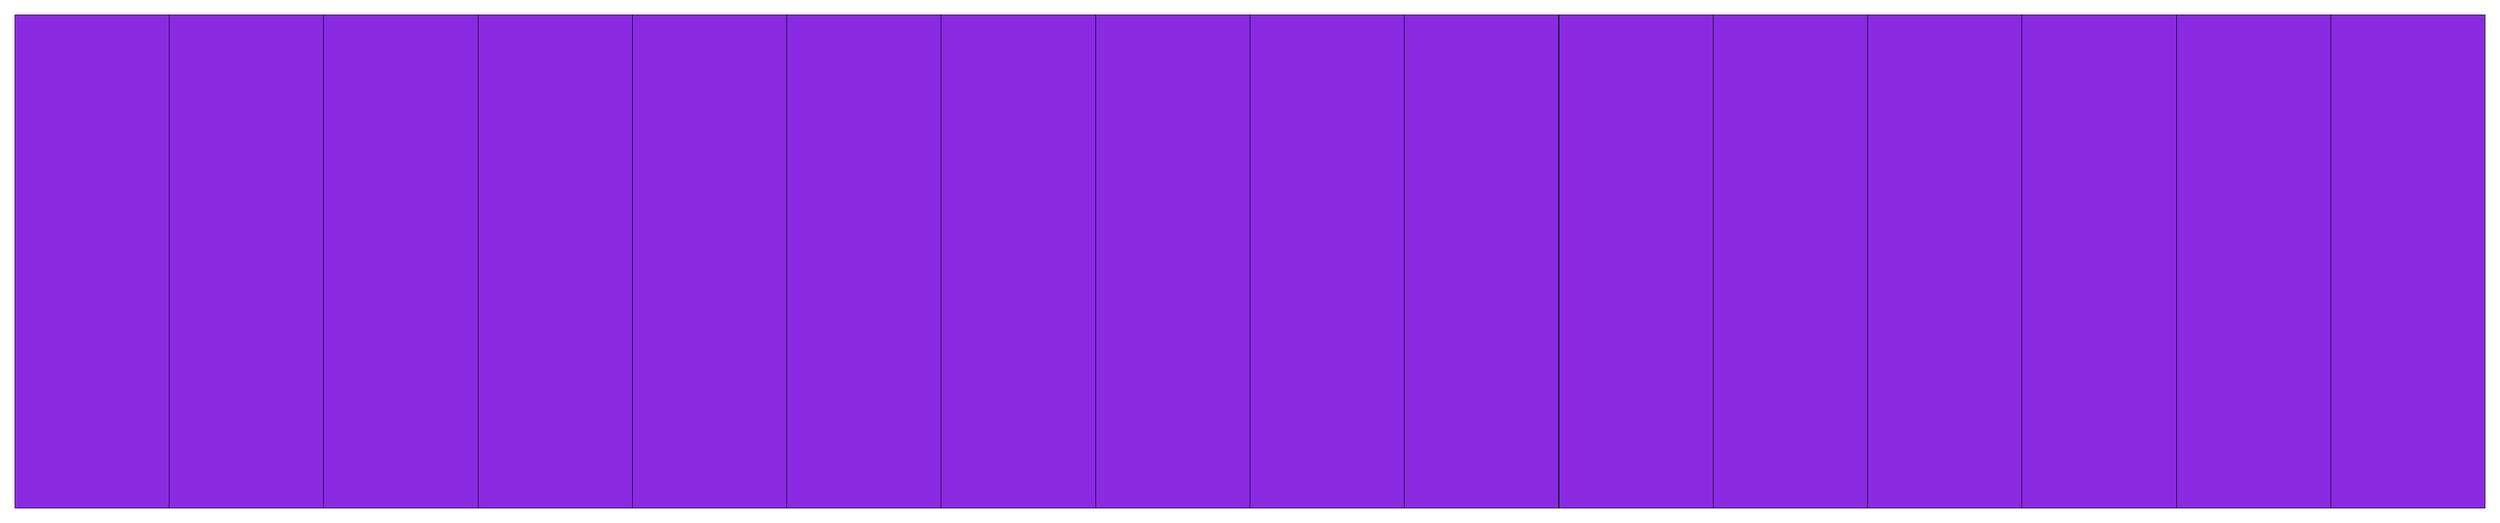
\begin{tikzpicture}
\draw[fill=BlueViolet] (0,0) rectangle (60,12);
\foreach \x in {1,...,15} \draw (\x*60/16,0) -- (\x*60/16,12);
\end{tikzpicture}}        &  \parbox[t][1.3 cm][c]{.2cm}{ }    &     \\
\hline
\end{longtable}
\end{center}
\vspace*{-1.1cm}

{\bf PARTE 2}

O objetivo desta parte é estudar a fração do retângulo que está colorida de cinza no segundo encarte que você recebeu.
\begin{center}
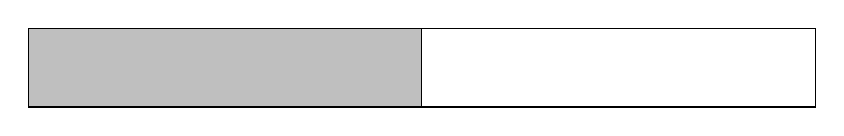
\begin{tikzpicture}[x=1mm, y=1mm]
% Fita principal (metade cinza, metade branca)
\draw (0,0) rectangle (100,10);
\draw[fill=lightgray] (0,0) rectangle (100/2,10);
\end{tikzpicture}
\end{center}

Para isto, responda às perguntas na tabela a seguir com frações adequadas. Se necessário, recorte e use as peças coloridas do primeiro encarte para avaliar as suas respostas.


\noindent  \begin{longtable}{|m{.35\textwidth}|m{.16\textwidth}|m{.18\textwidth}|m{.19\textwidth}|}
\hline
\centering Tipo da peça &   Quantas peças como essa cabem na região cinza? &   As peças que você usou, juntas, são que fração do retângulo do encarte?  &  Que fração do retângulo do encarte não está colorida de cinza? \\
\hline    \hline
\parbox[c][2cm][c]{.3\textwidth}{
\begin{tikzpicture}[x=1mm, y=1mm]
% Fita de largura 1/2
\draw[fill=light] (0,0) rectangle (100/2,10);
\end{tikzpicture}} &  \parbox[t][1.3 cm][c]{.2cm}{ } &  &  \\
\hline
\parbox[c][2cm][c]{.3\textwidth}{
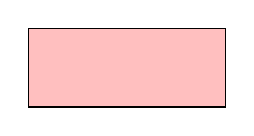
\begin{tikzpicture}[x=1mm, y=1mm]
% Fita rosa de largura 1/4
\draw[fill=pink] (0,0) rectangle (100/4,10);
\end{tikzpicture}}
&  \parbox[t][1.3 cm][c]{.2cm}{ } &  &  \\
\hline
\parbox[c][2cm][c]{.3\textwidth}{\begin{tikzpicture}[x=1mm, y=1mm]
% Fita rosa de largura 1/6
\draw[fill=special] (0,0) rectangle (100/6,10);
\end{tikzpicture}}    &  \parbox[t][1.3 cm][c]{.2cm}{ } &  &  \\
\hline
\parbox[c][2cm][c]{.3\textwidth}{\begin{tikzpicture}[x=1mm, y=1mm]
% Fita rosa de largura 1/8
\draw[fill=attention] (0,0) rectangle (100/8,10);
\end{tikzpicture}}     &  \parbox[t][1.3 cm][c]{.2cm}{ } &  &  \\
\hline
\parbox[c][2cm][c]{.3\textwidth}{\begin{tikzpicture}[x=1mm, y=1mm]
% Fita rosa de largura 1/10
\draw[fill=common] (0,0) rectangle (100/10,10);
\end{tikzpicture}}     &  \parbox[t][1.3 cm][c]{.2cm}{ } &  &  \\
\hline
\parbox[c][2cm][c]{.3\textwidth}{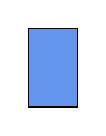
\begin{tikzpicture}[x=1mm, y=1mm]
% Fita rosa de largura 1/16
\draw[fill=CornflowerBlue] (0,0) rectangle (100/16,10);
\end{tikzpicture}}     &  \parbox[t][1.3 cm][c]{.2cm}{ } &  &  \\
\hline
\end{longtable}

\ifdefined\prof
\begin{solucao}


{\bf PARTE 1}
\vspace{1em}

\begin{center}
\begin{longtable}{|c|>{\centering}m{.25\textwidth}|>{\centering}m{.25\textwidth}|}
\hline
\centering Retângulo  &   Número de partes em que se encontra dividido  &   Cada parte é que fração do retângulo?  \tabularnewline
\hline
\endhead
\parbox[c][2cm][c]{.4\textwidth}{
\centering
\begin{tikzpicture}
\draw[fill=light] (0,0) rectangle (60,12);
\draw (30,0) -- (30,12);
\end{tikzpicture}}   &   \centering $2$ &  \centering $\dfrac{1}{2}$  \tabularnewline
\hline
\parbox[c][2cm][c]{.4\textwidth}{
\centering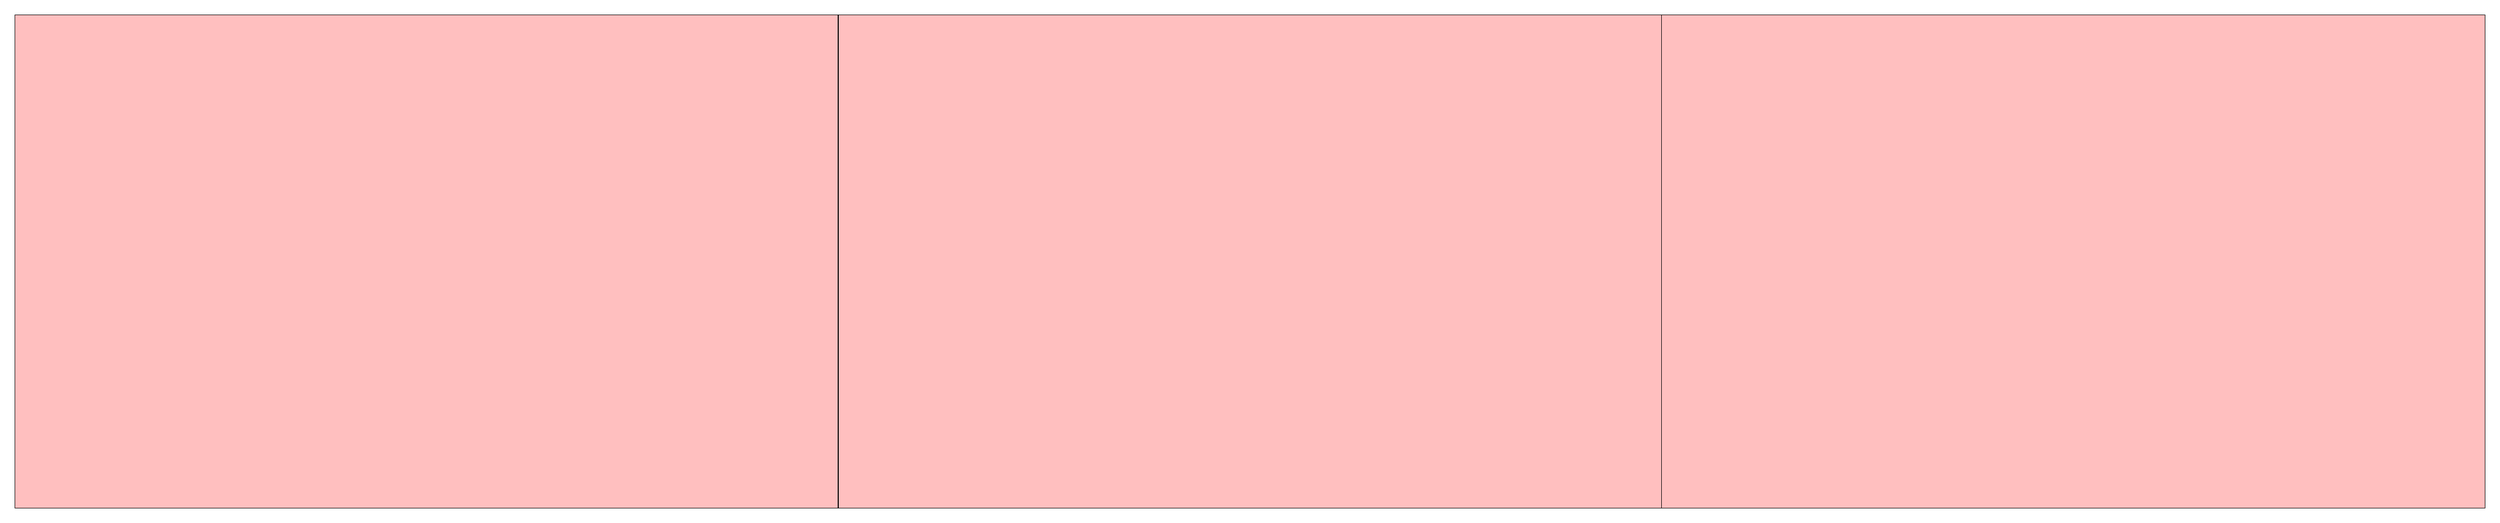
\begin{tikzpicture}
\draw[fill=pink] (0,0) rectangle (60,12);
\foreach \x in {1,2} \draw (\x*60/3,0) -- (\x*60/3,12);
\end{tikzpicture}}        &   $3$   &  $\dfrac{1}{3}$   \tabularnewline
\hline
\parbox[c][2cm][c]{.4\textwidth}{
\centering\begin{tikzpicture}
\draw[fill=special] (0,0) rectangle (60,12);
\foreach \x in {1,2,3} \draw (\x*60/4,0) -- (\x*60/4,12);
\end{tikzpicture}}        &   $4$   &  $\dfrac{1}{4}$   \tabularnewline
\hline
\parbox[c][2cm][c]{.4\textwidth}{
\centering\begin{tikzpicture}
\draw[fill=attention] (0,0) rectangle (60,12);
\foreach \x in {1,...,4} \draw (\x*60/5,0) -- (\x*60/5,12);
\end{tikzpicture}}        &  $5$    &  $\dfrac{1}{5}$   \tabularnewline
\hline
\parbox[c][2cm][c]{.4\textwidth}{
\centering\begin{tikzpicture}
\draw[fill=common] (0,0) rectangle (60,12);
\foreach \x in {1,...,5} \draw (\x*60/6,0) -- (\x*60/6,12);
\end{tikzpicture}}        &   $6$   &  $\dfrac{1}{6}$   \tabularnewline
\hline
\parbox[c][2cm][c]{.4\textwidth}{
\centering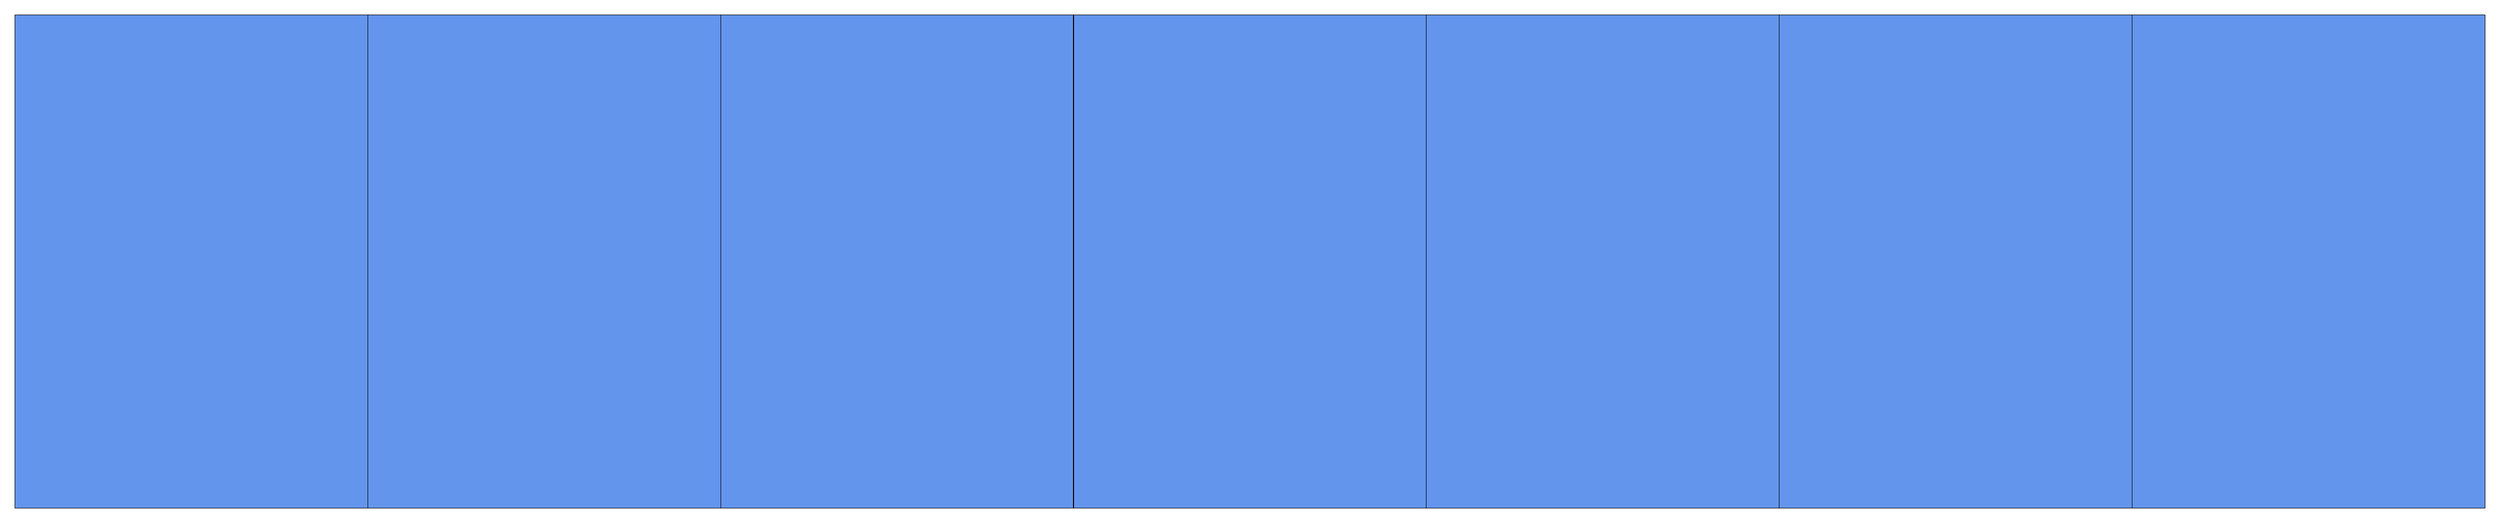
\begin{tikzpicture}
\draw[fill=CornflowerBlue] (0,0) rectangle (60,12);
\foreach \x in {1,...,6} \draw (\x*60/7,0) -- (\x*60/7,12);
\end{tikzpicture}}        &   $7$   &  $\dfrac{1}{7}$   \tabularnewline
\hline
\parbox[c][2cm][c]{.4\textwidth}{
\centering\begin{tikzpicture}
\draw[fill=dark] (0,0) rectangle (60,12);
\foreach \x in {1,...,7} \draw (\x*60/8,0) -- (\x*60/8,12);
\end{tikzpicture}}        &   $8$   &  $\dfrac{1}{8}$   \tabularnewline
\hline
\parbox[c][2cm][c]{.4\textwidth}{
\centering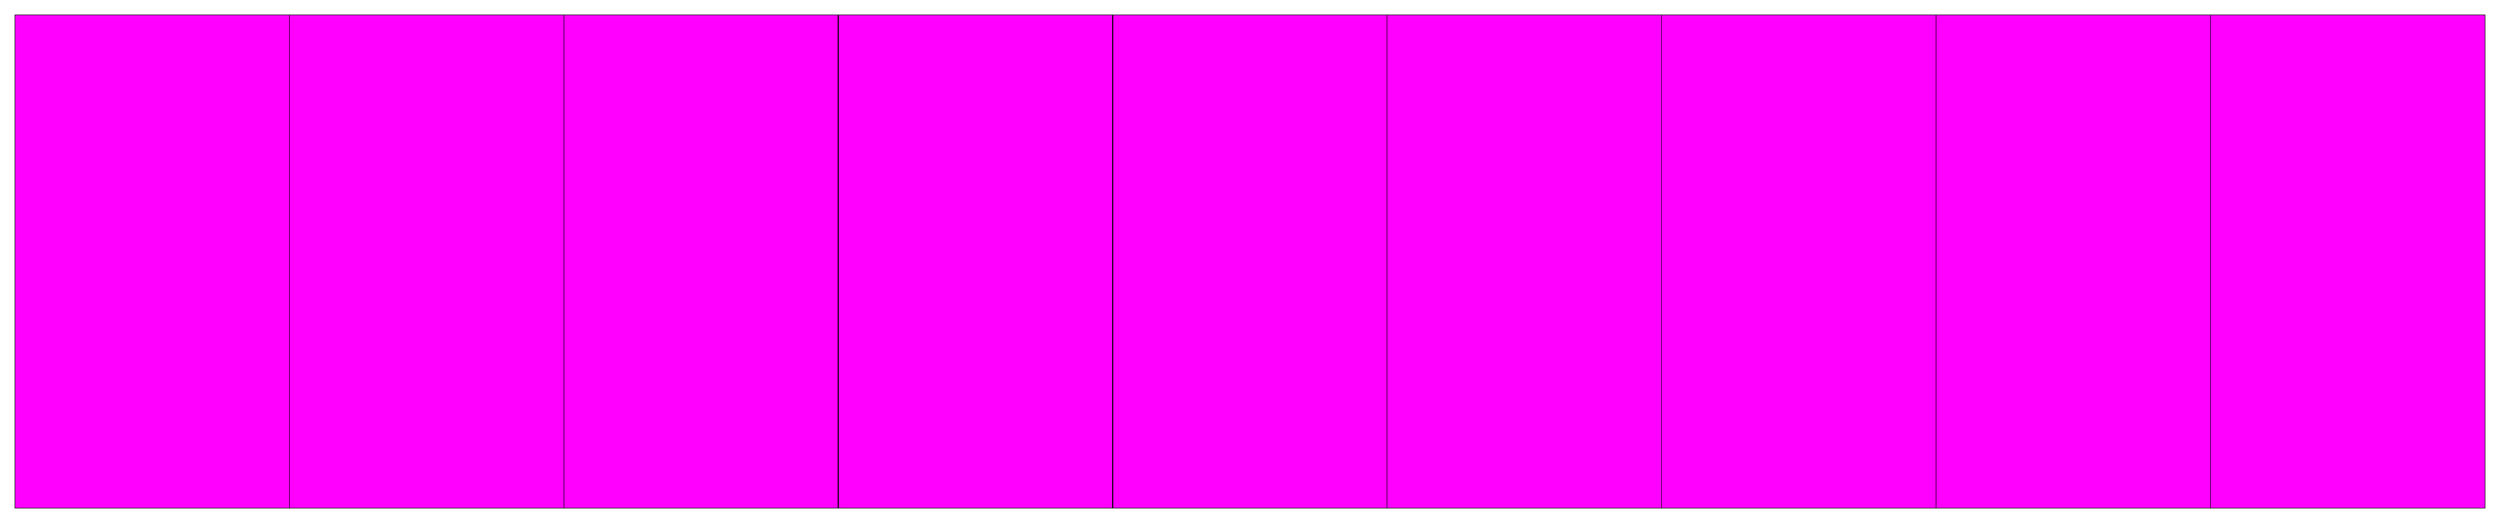
\begin{tikzpicture}
\draw[fill=Fuchsia] (0,0) rectangle (60,12);
\foreach \x in {1,...,8} \draw (\x*60/9,0) -- (\x*60/9,12);
\end{tikzpicture}}        &   $9$   &  $\dfrac{1}{9}$   \tabularnewline
\hline
\parbox[c][2cm][c]{.4\textwidth}{\centering
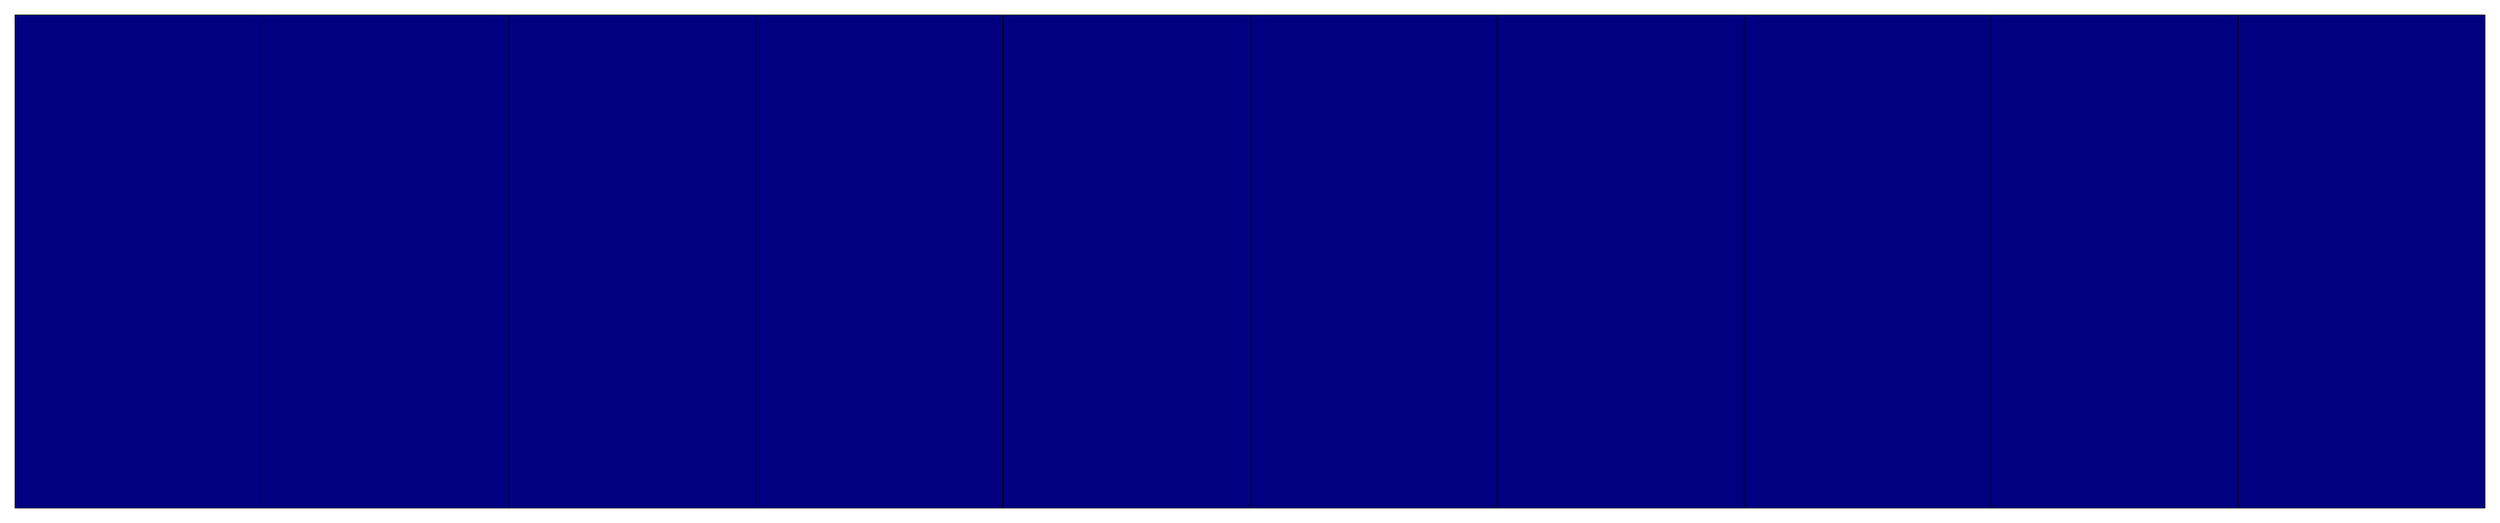
\begin{tikzpicture}
\draw[fill=NavyBlue] (0,0) rectangle (60,12);
\foreach \x in {1,...,9} \draw (\x*60/10,0) -- (\x*60/10,12);
\end{tikzpicture}}        &   $10$   &  $\dfrac{1}{10}$   \tabularnewline
\hline
\parbox[c][2cm][c]{.4\textwidth}{\centering
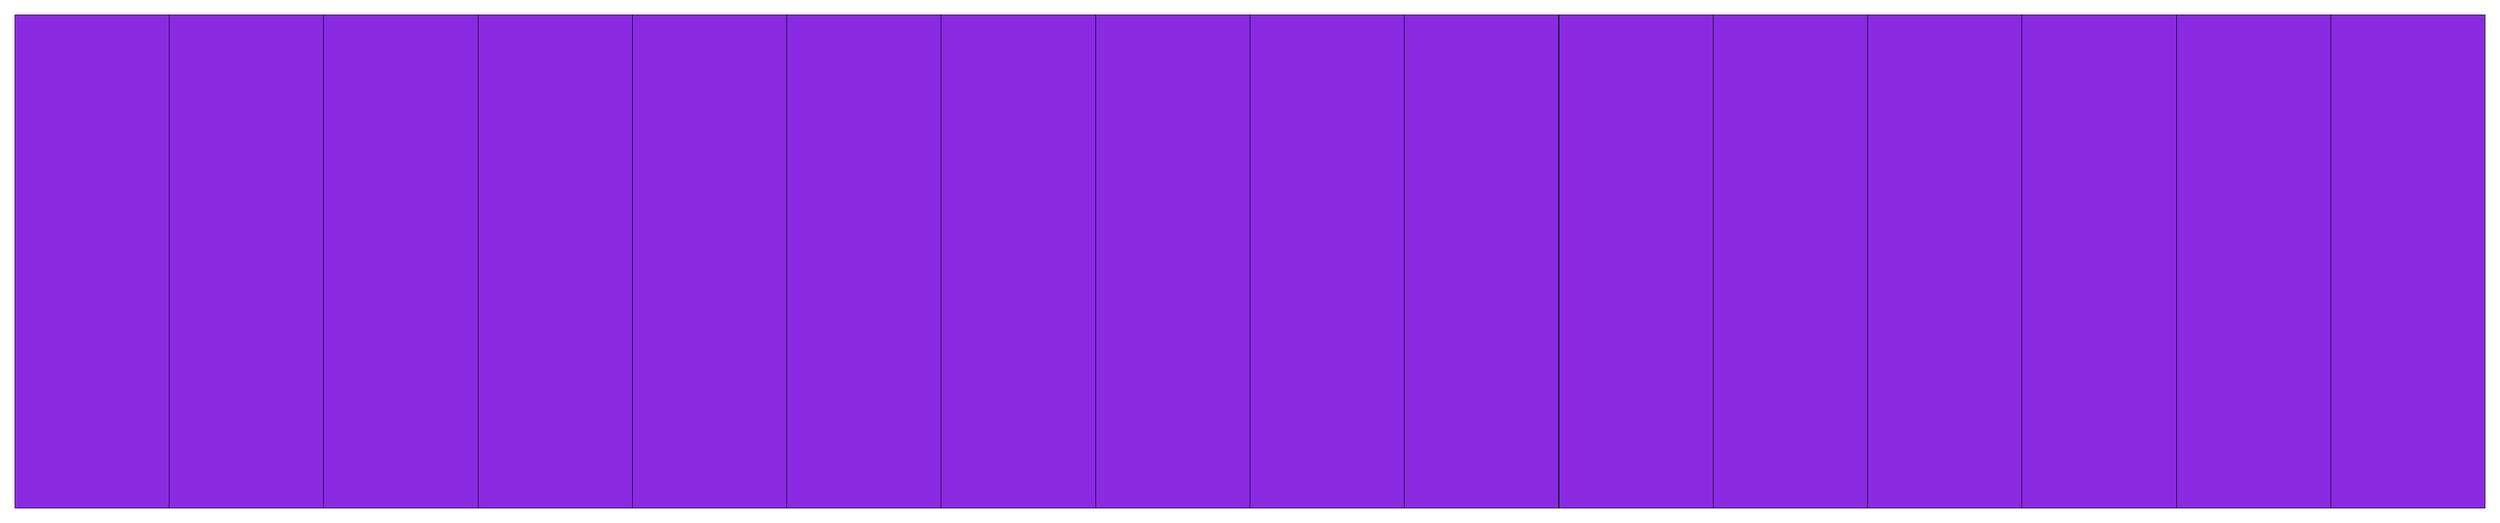
\begin{tikzpicture}
\draw[fill=BlueViolet] (0,0) rectangle (60,12);
\foreach \x in {1,...,15} \draw (\x*60/16,0) -- (\x*60/16,12);
\end{tikzpicture}}        &   $16$   &  $\dfrac{1}{16}$   \tabularnewline
\hline
\end{longtable}
\end{center}



  {\bf PARTE 2 }
\vspace{1em}

\noindent  \begin{longtable}{|m{.35\textwidth}|>{\centering}m{.16\textwidth}|>{\centering}m{.18\textwidth}|>{\centering}m{.19\textwidth}|}
\hline
\centering Tipo da peça &   Quantas peças como essa cabem na região cinza? &   As peças que você usou, juntas, são que fração do retângulo do encarte?  &  Que fração do retângulo do encarte não está colorida de cinza? \tabularnewline
\hline    \hline
\parbox[c][2cm][c]{.3\textwidth}{
\begin{tikzpicture}[x=1mm, y=1mm]
% Fita de largura 1/2
\draw[fill=light] (0,0) rectangle (100/2,10);
\end{tikzpicture}} &  $1$ & $\dfrac{1}{2}$ & $\dfrac{1}{2}$ \tabularnewline
\hline
\parbox[c][2cm][c]{.3\textwidth}{
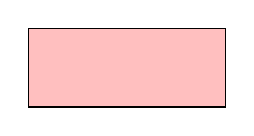
\begin{tikzpicture}[x=1mm, y=1mm]
% Fita rosa de largura 1/4
\draw[fill=pink] (0,0) rectangle (100/4,10);
\end{tikzpicture}}
&  $2$ & $\dfrac{2}{4}$ & $\dfrac{2}{4}$ \tabularnewline
\hline
\parbox[c][2cm][c]{.3\textwidth}{\begin{tikzpicture}[x=1mm, y=1mm]
% Fita rosa de largura 1/6
\draw[fill=special] (0,0) rectangle (100/6,10);
\end{tikzpicture}}    &  $3$ & $\dfrac{3}{6}$ & $\dfrac{3}{6}$ \tabularnewline
\hline
\parbox[c][2cm][c]{.3\textwidth}{\begin{tikzpicture}[x=1mm, y=1mm]
% Fita rosa de largura 1/8
\draw[fill=attention] (0,0) rectangle (100/8,10);
\end{tikzpicture}}     & $4$  & $\dfrac{4}{8}$ & $\dfrac{4}{8}$ \tabularnewline
\hline
\parbox[c][2cm][c]{.3\textwidth}{\begin{tikzpicture}[x=1mm, y=1mm]
% Fita rosa de largura 1/10
\draw[fill=common] (0,0) rectangle (100/10,10);
\end{tikzpicture}}     & $5$  & $\dfrac{5}{10}$ &  $\dfrac{5}{10}$ \tabularnewline
\hline
\parbox[c][2cm][c]{.3\textwidth}{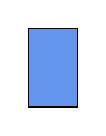
\begin{tikzpicture}[x=1mm, y=1mm]
% Fita rosa de largura 1/16
\draw[fill=CornflowerBlue] (0,0) rectangle (100/16,10);
\end{tikzpicture}}     & $8$  & $\dfrac{8}{16}$ & $\dfrac{8}{16}$ \tabularnewline
\hline
\end{longtable}

\end{solucao}
\fi

\end{document}